\chapter{ChordReduce}
\label{chapter:chordreduce}

Google's MapReduce \cite{mapreduce} paradigm has rapidly become an integral part in the world of data processing and is capable of efficiently executing numerous Big Data programming and data-reduction tasks.  By using MapReduce, a user can take a large problem, split it into small, equivalent tasks and send those tasks to other processors for computation.  The results are sent back to the user and combined into one answer.  Many popular platforms for MapReduce, such as Hadoop \cite{hadoop}, utilize a central source of coordination and organization to store and operate on data. The hierarchical structure of Hadoop results in a single point of failure at the node that concentrates the results and also requires a complicated scheme for handling node failures.

We developed a system, called ChordReduce, which employs a less hierarchical structure.  
It is a system that can scale, is fault tolerant, has a minimal amount of latency, and distributes tasks evenly.  ChordReduce leverages the underlying protocol from Chord \cite{chord} to distribute Map and Reduce tasks to nodes evenly, provide greater data redundancy, and guarantee a greater amount of fault tolerance. Rather than viewing Chord solely as a means for sharing files, we see it as a means for distributing work. This paper establishes the effectiveness of using Chord as a framework for distributed programming.   At the same time we avoid the architectural and file system constraints of systems like Hadoop.  


\section{Background}
ChordReduce takes its name from the two components it is built upon.  Chord \cite{chord} provides the backbone for the network and the file system, providing scalable routing, distributed storage, and fault-tolerance.   MapReduce runs on top of the Chord network and utilizes the underlying features of the distributed hash table.  This section provides background on Chord and MapReduce.


\subsection{Chord}
Chord \cite{Chord} is a P2P protocol for file sharing that uses a hash function to assign addresses to nodes and files for a ring overlay. The Chord protocol takes in some key and returns the identity (ID) of the node responsible for that key.  These keys are generated by hashing a value of the node, such as the IP address and port, or by hashing the filename of a file.  The hashing process creates a $m$-bit hash identifier.

The nodes are then arranged in a ring from the lowest hash-value to highest.  Chord takes the files and places each in the node that has the same hashed identifier as it.  If no such node exists, the node with the first identifier that follows this value is selected. Since the overlay is a circle, this assignment is computed in modulo $2^m$ space.  

The node responsible for the key $\kappa$ is called the $successor$ of $\kappa$, or $successor(\kappa)$.  For example, if there were some portion of the network with nodes 20, 25, and 27, node 25 would be responsible for the files with the keys (21,22,23,24,25). If node 25 were to decide to leave the network, its absence would be detected by node 27, who would then be responsible for all the keys node 25 was covering, in addition to its own keys. 
\begin{figure}
	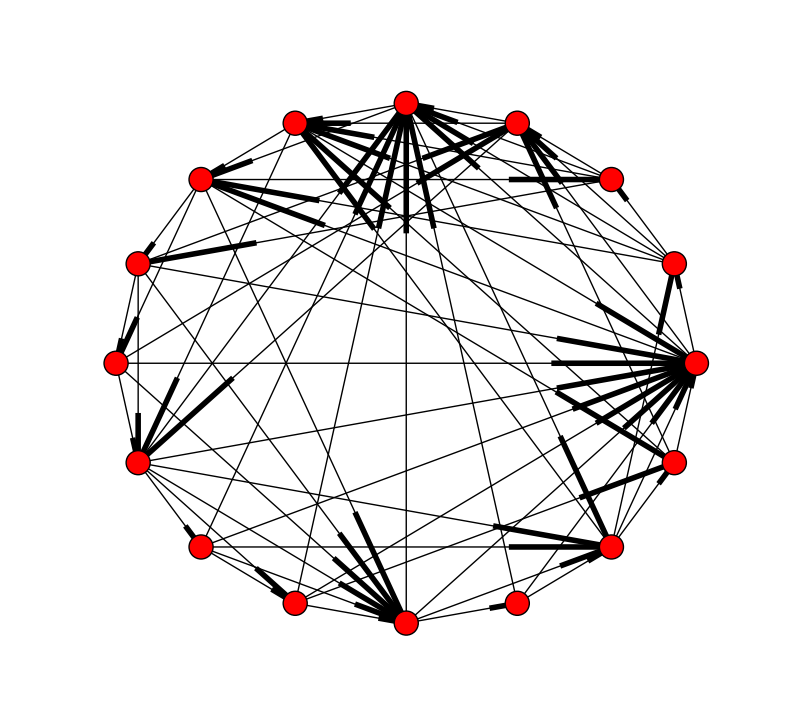
\includegraphics[width=\linewidth]{figs/chordreal}
	\caption{A Chord ring with 16 nodes.  The bold lines are incoming edges.  Each node has a connection to its successor, as well as 4 fingers, some of which are duplicates.}
	\label{fig:chordreal}
\end{figure}


With this scheme, we can reliably find the node responsible for some key by asking the next node in the circle for the information, who would then pass the request through the circle until the successor was found.  We can then proceed to directly connect with the successor to retrieve the file.  This naive approach is largely inefficient, and is a simplification of the lookup process, but it is the basis of how Chord theoretically works.

To speed up the lookup time, each node builds and maintains a \emph{finger table}.  The \emph{finger table} contains the locations of up to $m$ other nodes in the ring.  The $i$th entry of node $n$'s \emph{finger table} corresponds to the node that is the $successor(n+2^{i-1})$ $mod$ $2^m$. Hash values are not perfectly distributed, it is possible to have duplicate entries in the \emph{finger table}. An example Chord network with fingers is shown in in Fig. \ref{chordreal}.


\begin{figure}
	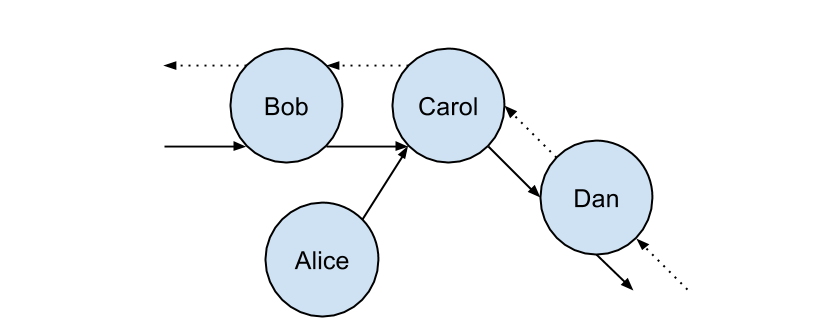
\includegraphics[width=\linewidth]{figs/abcd1}
	\caption{Alice has incorrectly determined that Carol is her appropriate successor.  When Alice stabilizes, Carol will let her know about Bob.}
	\label{fig:abcd1}
\end{figure}


\begin{figure}
	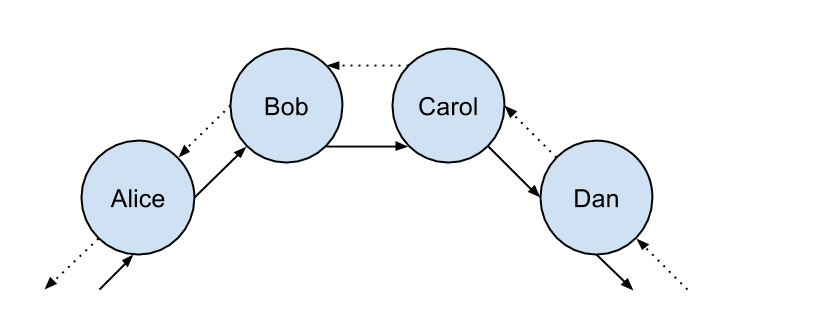
\includegraphics[width=\linewidth]{figs/abcd2}
	\caption{After completing stabilize, Alice makes Bob her successor and notifies him. Bob then made Alice as his predecessor.}
	\label{fig:abcd2}
\end{figure}



When a node $n$ is told to find some key, $n$ looks to see if the key is between $n$ and $successor(n)$ and return $successor(n)$'s information to the requester. If not, it looks for the entry in the finger table for the closest preceding node $n'$ it knows and asks $n'$ to find the successor.  This allows each step to skip up to half the nodes in the network, giving a $\log_2(n)$ lookup time.  Because nodes can constantly join and leave the network, each entry in the table is periodically checked and updated during a finger maintenance period. 

To join the network, node $n$ first asks $n'$ to find $successor(n)$ for it.  Node $n$ uses the information to set his successor, but the other nodes in the ring will not acknowledge $n$'s presence yet.  Node $n$ relies on the stabilize routine to fully integrate into the ring.

The stabilize routine helps the network integrate new nodes and route around nodes who have left the network. Each node periodically checks to see who their successor's predecessor is.  In the case of a static network, this would be the checking node.  However, if the checking node gets back a different node, it looks at that returned node's hash value and changes its own successor if needed.  Regardless of whether the checking node changes its successor, that node then notifies the (possibly) new successor,  who then checks if he needs to change his predecessor based on this new information.  While complex, the stabilization process is no more expensive than a heartbeat function.  A more concrete example:


Suppose Alice, Bob, Carol, and Dan are members of the ring and everyone is ordered alphabetically (Fig. \ref{abcd1}). Alice is quite sure that Carol is her successor.  Alice asks Carol who her predecessor is and Carol says Bob is.  Since Bob is closer than Carol, Alice changes her successor to Bob and notifies him.  

When Bob sees that notification, he can see Alice is closer than whoever his previous predecessor is and sets Alice to be his predecessor.  During the next stabilization cycle, Alice will see that she is still Bob's predecessor and notify him that she's still there (Fig. \ref{fig:abcd2}).

To prevent loss of data due to churn, each node sends a backup of their data to their successor.  Section IV discusses the implementation of the backup process in ChordReduce and expands upon it for backing up Map and Reduce tasks.


\subsection{Extensions of Chord}

The Cooperative File System (CFS) is an anonymous, distributed file sharing system built on top of Chord \cite{CFS}.  In CFS, rather than storing an entire file at a single node, the file is split up into multiple chunks around 10 kilbytes in size.  These chunks are each assigned a hash and stored in nodes corresponding to their hash in the same way that whole files are.  The node that would normally store the whole file instead stores a \emph{key block}, which holds the hash address of the chunks of the file. 

The chunking allows for numerous advantages.  First, it promotes load balancing. Each piece of the overall file would (ideally) be stored in a different node, each with a different backup or backups.  This would prevent any single node from becoming overwhelmed from fulfilling multiple requests for a large file.  It would also prevent retrieval from being bottlenecked by a node with a relatively low bandwidth. Finally, when Chord uses some sort of caching scheme like that described in CFS \cite{CFS}, caching chunks as opposed to the entire file resulted in about 1000 times less storage overhead.  

Mutable files  and  IRM, which is short for Integrated File Replication and Consistancy Maintenence, has nodes keep track of file requests they initiate or forward.  If they find they are frequently forwarding a request for a particular file, they store that file locally until it is no longer requested frequently.  What makes IRM unqiue is that it combines caching with a 

Chunking also opens up the options for implementing additional redundancy such as erasure codes \cite{rizzo1997effective}. With erasure codes, redundant chunks are created but any combination of a particular number of chunks is sufficient to recreate the file.  For example, a file that would normally be split into 10 chunks might be split into 15 encoded chunks.  The retreival of any 10 of those 15 chunks is enough to recreate the file.  Implementing erasure codes would presumably make the network more fault tolerant, but that is an exercise left for future work.


Generally, related files should be kept together; Chord, however, just hashes the filename to find the responsible node and sends it to that location without any thought to organization.  Our solution to this is to use allow the file owner to select first 80 bits of a file's hash, then generating the remaining least signifcant bits by hashing the filename.  It does not matter if a file owner, in some infintesimally small coincidence, chooses the same 80 bit prefix as another file owner, as the purpose is to keep related files together.   